%FOR PDFLATEX USE ONLY
\documentclass[a4paper,14pt]{article}

\usepackage{amssymb,amsmath} %math symbols

\usepackage[margin=2cm, bottom=2cm]{geometry} %paper geometry

\usepackage[utf8]{inputenc} %allows unicode (including russian) source file
\usepackage[russian]{babel} %docment in russian-style
\usepackage[utf8]{inputenc}
\usepackage[unicode]{hyperref} %links inside of the text
\usepackage[pdftex]{graphicx} %includegraphics pictures
\usepackage{cmlgc} %bold text

\usepackage{array} %arrays

\usepackage{cancel}
\usepackage{wrapfig}
\usepackage{array}
\usepackage{lipsum}
\usepackage{esvect}
\usepackage{longtable}
\usepackage{verbatim} 
\usepackage{multirow}
\usepackage{hyperref}
\usepackage{mathtools}
\usepackage{subfig}
\usepackage{calc}
\usepackage{pgfplots,tikz,circuitikz}
\usepackage{tkz-euclide}

\newenvironment{changemargin}[2]{%
\begin{list}{}{%
\setlength{\topsep}{0pt}%
\setlength{\leftmargin}{#1}%
\setlength{\rightmargin}{#2}%
\setlength{\listparindent}{\parindent}%
\setlength{\itemindent}{\parindent}%
\setlength{\parsep}{\parskip}%
}%
\item[]}{\end{list}}

\newcommand{\specialcell}[2][c]{%
  \begin{tabular}[#1]{@{}c@{}}#2\end{tabular}}
%\newenvironment{comment}{}{}

\begin{document}
\section*{1.4}
\begin{center}
	Последовательность событий в космологии. \\
	Возраст вселенной по разным данным $13.75 \pm 0.13$ (WMAP) или $13.81 \pm 0.06$ (Planck) гигалет.
\end{center}
\begin{center}
\begin{longtable}{|c|c|c|}
\hline
 Время& Эпоха& События\\
\hline
 0& Сингулярность& Большой взрыв\\
\hline
 0 — $10^{-43}$ с& Планковская эпоха& Рождение частиц\\
\hline
 $10^{-43}$ — $10^{-35}$ с & \specialcell{Эпоха Великого\\объединения}& \specialcell{Отделение гравитации от\\ объединённого электрослабого\\ и сильного взаимодействия.\\ Возможное рождение\\ монополей. Разрушение\\ Великого объединения.} \\
\hline
 $10^{-35}$ — $10^{-32}$ с& Инфляционная эпоха& \specialcell{Вселенная экспоненциально\\ увеличивает свой радиус на\\ много порядков. Структура\\ первичной квантовой\\ флуктуации, раздуваясь, даёт\\ начало крупномасштабной\\ структуре Вселенной.\\ Вторичный нагрев.} \\
\hline
 $10^{-32}$ — $10^{-12}$ с& Электрослабая эпоха& \specialcell{Вселенная заполнена кварк-\\глюонной плазмой, лептонами,\\ фотонами, W- и Z-бозонами,\\ бозонами Хиггса. Нарушение\\ суперсимметрии.} \\
\hline
 $10^{-12}$ — $10^{-6}$ с& Кварковая эпоха& \specialcell{Электрослабая симметрия\\ нарушена, все четыре\\ фундаментальных\\ взаимодействия существуют\\ раздельно. Кварки ещё не\\ объединены в адроны.\\ Вселенная заполнена кварк-\\глюонной плазмой, лептонами и\\ фотонами.} \\
\hline
 $10^{-6}$ — 100 с& Адронная эпоха& \specialcell{Адронизация. Аннигиляция\\ барион-антибарионных пар.\\ Благодаря CP-нарушению\\ остаётся малый избыток\\ барионов над антибарионами\\ (около 1:$10^9$).} \\
\hline
 100 секунд — 3 минуты& Лептонная эпоха& \specialcell{Аннигиляция лептон-\\антилептонных пар. Распад\\ части нейтронов. Вещество\\ становится прозрачным для\\ нейтрино.} \\
\hline
 3 минуты — 380 000 лет& Протонная эпоха& \specialcell{Нуклеосинтез гелия, дейтерия,\\ следов лития-7 (20 минут).\\ Вещество начинает\\ доминировать над излучением\\ (70 000 лет), что приводит к\\ изменению режима расширения\\ Вселенной. В конце эпохи (380\\ 000 лет) происходит\\рекомбинация водорода и\\ Вселенная становится\\ прозрачной для фотонов\\ теплового излучения.} \\
\hline
 380 000 — 550 млн лет& Тёмные века& \specialcell{Вселенная заполнена\\ водородом и гелием,\\ реликтовым излучением,\\ излучением атомарного\\ водорода на волне 21 см.\\ Звёзды, квазары и другие яркие \\источники отсутствуют.} \\
\hline
 (550 — 800) млн лет& Реионизация& \specialcell{Образуются первые звёзды\\ (звёзды популяции III), квазары,\\ галактики, скопления и\\ сверхскопления галактик.\\ Реионизация водорода светом\\ звёзд и квазаров.} \\
\hline
 (0.8 — 8.9) млрд лет& Эра вещества& \specialcell{Образование межзвёздного\\ облака, давшего начало\\ Солнечной системе.} \\
\hline
 (8.9 — 9.1) млрд лет& Эра вещества& \specialcell{Образование Земли и других\\ планет нашей Солнечной\\ системы, затвердевание пород.} \\
\hline
\end{longtable}
\end{center}
\section*{1.7}
\begin{center}
	Почему выживают мутации (не растворяются в популяции). \\
\end{center}
Для начала стоит отметить, что постановка вопроса некорректна, так как существуют мутации, которые вызывают быструю гибель организма, и таким образом мутация очень быстро вымывается из популяции. К таким можно отнести доминантные летальные мутации.
Другое дело - рецессивные летальные мутации. Они очень устойчивы, и это крайне легко показать, используя общие соображения и закон Харди-Вайнберга:
\begin{equation*}
p^2 + 2pq + q^2 = 1.
\end{equation*}
Отбор против рецессивной гомозиготы - пускай до полового созревания умрет w процентов особей с таким генотипом. Тогда рассчитаем изменение частоты аллеля a рассматриваемого гена за одно поколение: 
\begin{equation*}
q1 = (q - pq^2) / (1 - wq^2), p1 =  p / (1 - wq^2),\\
\end{equation*}
\begin{equation*}
\Delta q = q1 - q =  - wpq^2  / (1 -wq^2).
\end{equation*}
Нормализованные частоты:
\begin{equation*}
(aa)  q^2=q^2(1-w)/(1-wq^2),\;\;\;\;\;\;\;\;\;\;(Aa) 2pq=2pq/ (1-wq^2),\;\;\;\;\;\;\;\;\;\;(AA) p^2=p^2/(1-wq^2).
\end{equation*}
Пользуясь этой формулой, можно рассчи­тать, например, как будет убывать в популяции частота встреча­емости летального рецессивного гена, вызывающего 100-процентную смертность гомозигот аа. Оказывается, что даже при столь жестком отборе смертоносный рецессивный ген сохраняется сотни поколений, выщепляясь постепенно из гетерозигот.
\begin{center}
	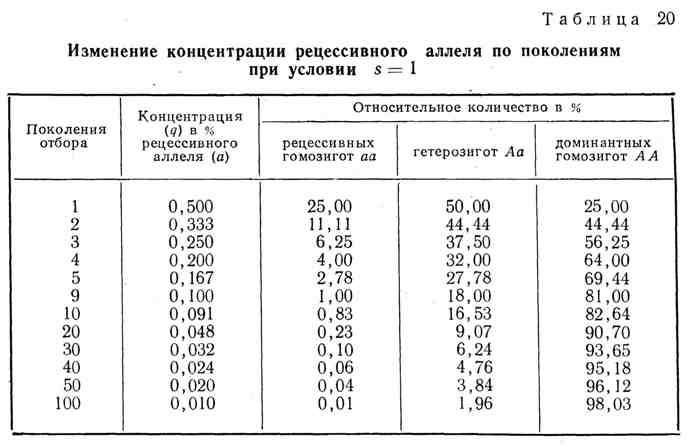
\includegraphics[width=0.80\textwidth]{img/1_7_0.png}
\end{center}
\section*{2.3}
\begin{center}
	Элементарные частицы и их свойства. \\
\end{center}
\begin{scriptsize}
\begin{center}
\begin{tabular}{cccccccc}
\hline
& Электрический & Цветной & Барионное& Спин & Магнитный  & Изоспин & Внутренняя\\
& заряд &заряд& число & & момент  && четность\\
Протон & +1 &"белый"& 1 &  1/2 & 1,41060679736(60)$\cdot10^{-26}$  & 1/2& 1\\
Нейтрон & 0 &"белый"& 1 &  1/2 & -9,6623651(23)$\cdot10^{-27}$ & -1/2& 1\\
\hline
& Электрический &Цветной& Барионное& Спин & Слабый & Изоспин& Четность\\
& заряд &заряд& число & & гиперзаряд && \\
Пион &$\pm1$ & "белый"&0&0&0, -2, -1&$\pm1$& -
\\
\hline
& Электрический &Цветной& Лептонное & Спин & Магнитный && Внутренняя   \\
& заряд &заряд& число & & момент && четность\\
Электрон & -1 &0 & 1 & 1/2 & -9,274009994(57)$\cdot10^{-24}$ && 1
\\
\hline
& Электрический &Цветной& Лептонное & Спин &&& \\
& заряд & заряд & число &&&&  \\
Мюон & -1 &0& 1 & 1/2 &&&
\\
\hline
& Электрический &Цветной& Лептонное & Спин & Кол-во спиновых   \\
& заряд &заряд& число & & состояний \\
$\tau$-лептон & -1 &0& 1 & 1/2 & 2
\\
\hline
& Электрический &Цветной& Лептонное & Спин & Слабый  \\
& заряд &заряд& число & & гиперзаряд \\
Нейтрино & 0 & 0 & 1 & 1/2 & -1
\\
\hline
& Электрический &Цветной& Барионное & Спин  \\
& заряд &заряд& число & \\
Кварк & кратен e/3 & r, g, b & 1/3 & 1/2 
\\
\hline
& Электрический & Цветной && Спин & Количество спиновых  \\
& заряд & заряд &&& состояний\\
W$^+$- базон & +1& 0&& 1&3\\
W$^-$- базон& -1 &0 &&1&3\\
Z -  базон&0 &0 && 1&3\\
\hline
& Электрический &Цветной&& Спин &Кол-во спиновых&& Внутренняя\\
& заряд &заряд&& & Состояний&& четность \\
Глюон& 0& $r\bar r, g\bar g, b\bar b, r\bar g, r\bar b, g\bar b$,&& 1& 2&& -
\\
\hline
&Эликтрический& Цветной&& Спин& Кол-во спиновых& Спиральность& Внутренняя\\
&заряд& заряд&&& состояний&&четность\\
Фотон &0& 0&& 1& 2& $\pm$1& -
\\
\hline
&Электрический& Цветной&& Спин&&& Четность\\
&заряд& заряд\\
Базон Хиггса &0& 0&& 0&&& +1\\
\hline
\end{tabular}
\end{center}
\end{scriptsize}

Электрический заряд - квантовое число, определяющее способность частиц принимать участие в электромагнитном взаимодействие.\\
Цветной заряд — квантовое число, приписываемое глюонам и кваркам, которые участвуют в сильном взаимодействии. Цветов три: «красный», «зелёный» и «синий», хотя эти названия не имеют никакого отношения к цветам, которые мы видим в повседневной жизни, также существуют три антицвета.\\
Спин — собственный момент импульса элементарных частиц. Спин измеряется в единицах $\hbar$ (постоянной Дирака) и равен $\hbar$J, где J — характерное для каждого сорта частиц целое или полуцелое положительное число — так называемое спиновое квантовое число, которое и приведено в таблице.\\
Изоспин — квантовое число, определяющая число зарядовых состояний адронов.\\
Магнитный момент — квантовое число, характеризующее магнитные свойства частицы. Измеряется в Дж/Тл.\\
Барионное число — квантовое число, определяющее количество барионов (элементарных частиц, состоящих из трёх кварков) в системе.\\
Лептонное число — разность числа лептонов (частиц с полуцелым спином, не участвующих в сильном взаимодействии) и антилептонов в данной системе.\\
Спиральность — квантовое число, используемое при описании элементарных частиц, движущихся со скоростью света или близкой к ней.

\section*{3.9}

\begin{center}
	Исследование вынужденной регулярной прецессии гироскопа.\\
\end{center}

Оценим время, которое требуется фотону, чтобы вылететь из Солнца, таким образом: положим томсоновское рассеяние на свободном электроне самым распространённым типом рассеяния фотонов в недрах Солнца, его эффективное сечение $\sigma = 7 \cdot 10^{-29} \text{ м}^2$.

Для оценки положим концентрацию электронов $n_e$ не зависящей от глубины. Длина свободного пробега фотона $\lambda = \frac{1}{n_e \sigma} = 2 \text{ см}$.

Вследствие многократного рассеяния, путь фотона выглядит как случайное блуждание. Тогда время, за которое фотон переместится на радиус Солнца $R$, читается так:
$T = \frac{R^2}{\lambda c} = 10^3 \text{ лет}.$

Полученная оценка является несколько заниженной. В действительности, конечно, томсоновский механизм реализуется в глубоких слоях Солнца, где концентрация электронов существенно выше средней, а при более низких температурах возможны более эффективные взаимодействия с веществом.

Источник: задача со сборов к международной олимпиаде по астрофизике.

\section*{4.3}

\begin{center}
	Лагранжиан стандартной модели.\\
\end{center}

\begin{equation*}
L = -\frac{1}{4} F_{\mu \nu} F^{\mu \nu} + i \overline{\psi} \cancel D \psi + h.c. + \psi_{i} y_{ij} \psi_{j} \phi + h.c. + |D_{\mu} \phi |^2 - V(\phi )
\end{equation*}

\section*{4.4}

\begin{center}
	Чем отличается темная материя от темной энергии?\\
\end{center}

Тёмная материя — гипотетическая форма материи, не участвующая в электромагнитном взаимодействии и поэтому недоступная прямому наблюдению. Составляет порядка четверти массы-энергии Вселенной и проявляется только в гравитационном взаимодействии. Понятие тёмной материи введено для теоретического объяснения проблемы скрытой массы в эффектах аномально высокой скорости вращения внешних областей галактик и гравитационного линзирования (в них задействовано вещество, масса которого намного превышает массу обычной видимой материи); среди прочих предложенных оно наиболее удовлетворительно.\\

Тёмная энергия — гипотетический вид энергии, введённый в математическую модель Вселенной ради объяснения наблюдаемого её расширения с ускорением.
Существует три варианта объяснения сущности тёмной энергии:
\begin{enumerate}
	\item тёмная энергия есть космологическая константа — неизменная энергетическая плотность, равномерно заполняющая пространство Вселенной (другими словами, постулируется ненулевая энергия и давление вакуума).
	\item тёмная энергия есть некая квинтэссенция — динамическое поле, энергетическая плотность которого может меняться в пространстве и времени.
	\item тёмная энергия есть модифицированная гравитация на расстояниях порядка размера видимой части Вселенной.
\end{enumerate}

\section*{4.7}

\begin{center}
	Конформационная структура белка - разные уровни и их роль.\\
\end{center}

Последовательность аминокислотных остатков в полипептидной цепи называется первичной структурой белка.
Цепочка из аминокислот не будет находиться в растворе в полностью вытянутой форме, обычно она складывается в более сложные структуры. Кислород группы C=O может образовывать водородную связь с водородом группы N-H, расположенной в другой аминокислоте. За счёт таких водородных связей формируется вторичная структура белка.\\
Укладка белков обычно не ограничивается вторичной структурой. Между аминокислотными остатками возникают различные слабые связи. Например, между -СОО$^-$-группами кислых аминокислот и NH3$^+$-группами лизина может возникнуть электростатическое притяжение. Между атомами кислорода или азота одних гидрофильных аминокислот и атомами водорода других могут образоваться водородные связи. Гидрофобные аминокислотные остатки "стремятся" укрыться от водного окружения внутри белковой молекулы. Некоторую роль играют также ван-дер-ваальсовы взаимодействия (они обеспечивают слабое притяжение любых атомов с электронными оболочками). Имеются и ковалентные связи, стабилизирующие третичную структуру белка, - это т. н. дисульфидные мостики -S-S-, образующиеся между двумя остатки аминокислоты цистеина: R-SH + R-SH - 2H = R-S-S-R. Благодаря всем этим взаимодействиям - гидрофобным, ионным, водородным, ван-дер-ваальсововым и дисульфидным - белковая цепочка образует сложную пространственную конфигурацию, называемую третичной структурой.\\
Многие белки (их называют олигомерными) состоят не из одной, а из нескольких полипептидных цепочек – так, белок крови гемоглобин состоит из четырех цепей. Совокупность их образует четвертичную структуру белка, при этом отдельные цепочки называются субъединицами. Четвертичная структура удерживается теми же связями, что и третичная. Пространственная конфигурация белка (т. е. его третичная и четвертичная структура) называется конформацией. Все более высокие уровни организации белковой молекулы определяются первичной структурой данного белка (постулат Полинга-Афинсена).

%\section*{4.9}

%\begin{center}
%	Что такое джозефсоновский контакт?\\
%\end{center}

%Туннельный эффект - это типичная задача квантовой механики. Частица (например, электрон в металле) подлетает к барьеру (например, к слою диэлектрика), преодолеть который она по классическим представлениям никак не может, так как ее кинетическая энергия недостаточна, хотя в области за барьером она со своей кинетической энергией вполне могла бы существовать. Напротив, согласно квантовой механике, прохождение барьера возможно. Частица с некоторой вероятностью может как бы пройти по туннелю через классически запрещенную область, где ее потенциальная энергия как бы больше полной, то есть классическая кинетическая энергия как бы отрицательна. На самом деле с точки зрения квантовой механики для микрочастицы (электрона) справедливо соотношение неопределенностей $\Delta x \Delta p > h$ (x - координата частицы, p - ее импульс). Когда малая неопределенность ее координаты в диэлектрике $\Delta x = d$ (d-толщина слоя диэлектрика) приводит к большой неопределенности ее импульса $\Delta p \ge h / \Delta x$, а следовательно, и кинетической энергии $p^2/(2m)$ (m - масса частицы), то закон сохранения энергии не нарушается. Опыт показывает, что действительно между двумя металлическими обкладками, разделенными тонким слоем диэлектрика (туннельный переход), может протекать электрический ток тем больший, чем тоньше диэлектрический слой.\\
%Джозефсон рассматривал частный случай туннельного эффекта - туннелирование куперовских пар - и предсказал существование двух эффектов. Первый из них состоит в том, что через туннельный переход с тонким слоем диэлектрика, когда его толщина меньше или порядка длины когерентности,  возможно протекание сверхпроводящего тока, то есть тока без сопротивления. Это стационарный эффект Джозефсона. Предсказывалось, что критическое значение этого тока будет своеобразно зависеть от внешнего магнитного поля. Если ток через такой переход станет больше критического, то переход будет источником высокочастотного электромагнитного излучения. Это нестационарный эффект Джозефсона.\\
%Понадобилось немного времени, чтобы обнаружить эти эффекты экспериментально. Более того, вскоре стало ясно, что эффекты Джозефсона присущи не только туннельным переходам, но и более широкому классу объектов - сверхпроводящим слабым связям, то есть участкам сверхпроводящей цепи, в которых критический ток существенно подавлен, а размер участка порядка длины когерентности.\\
%В основе эффектов Джозефсона лежат квантовые свойства сверхпроводящего состояния. Действительно, сверхпроводящее состояние характеризуется когерентностью куперовских пар: эти пары электронов находятся на одном квантовом уровне и описываются общей для всех пар волновой функцией, ее амплитудой и фазой. Они когерентны как частицы света - фотоны в излучении лазера, которое также характеризуется амплитудой и фазой электромагнитной волны.\\
%Представим теперь себе два массивных куска одного и того же сверхпроводника, полностью изолированных друг от друга. Так как оба они находятся в сверхпроводящем состоянии, каждый из них будет характеризоваться своей волновой функцией. Поскольку материалы и температуры одинаковы, модули обеих волновых функций должны совпадать, а фазы произвольны. Однако, если установить между ними хотя бы слабый контакт, например туннельный, куперовские пары будут проникать из одного куска в другой и установится фазовая когерентность. Возникнет единая волновая функция всего сверхпроводника, которую можно рассматривать как результат интерференции волновых функций двух половинок.



\end{document}